\subsubsection{A* con EXL}
\lezione{Lezione 6}{17/10/2024}
Dal momento che A* può essere visto come una generalizzazione di UCS (UCS è il caso in cui l'euristica è sempre nulla), possiamo
equipaggiare anche A* con una lista delle espansioni per ottimizzare il tempo di ricerca. Purtroppo, in questo caso, non è sempre detto
che con la EXL e l'euristica si conservi sempre l'ottimalità (perchè è possibile che si selezionino prima percorsi da espandere più lunghi di altri) ed è
per questo che l'euristica $h$ debba essere anche \textbf{consistente}.

\paragraph{Euristica Consistente}
La consistenza (o monotonicità) di un'euristica è una proprietà più forte dell'ammissibilità (quindi la implica) e afferma che:\\
Dati 2 nodi $V,U$ e un'azione $a$, allora
\begin{equation}
    h(V) \leq c(V,a,U) + h(U) \mbox{  } \forall V,U
\end{equation}
La proprietà può essere interpretata come una disuguaglianza triangolare in questa forma (G è il nodo goal):
\begin{center}
    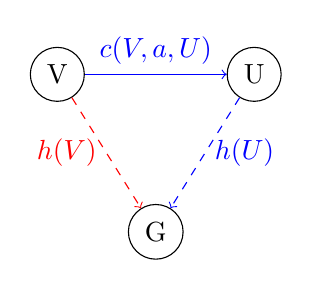
\begin{tikzpicture}
        % Nodi
        \node[circle, draw] (V) at (0,0) {V};
        \node[circle, draw] (U) at (2.5,0) {U};
        \node[circle, draw] (G) at (1.25,-2) {G};

    
        % Archi
        \draw[->, blue] (V) -- (U) node[midway, above] {$c(V,a,U)$}; % Arco da A a B
        \draw[->, dashed, red] (V) -- (G) node[midway, left] {$h(V)$}; % Arco da B a D
        \draw[->, dashed, blue] (U) -- (G) node[midway, right] {$h(U)$}; % Arco da D a C

    
    \end{tikzpicture}
\end{center}
Ossia, la stima di un nodo non può essere peggiore del costo per arrivare al nodo successivo + la stima del nodo successivo.

\subsubsection{Monotonicità di $f$}
Assumendo che $h$ sia consistente, allora possiamo dimostrare che $f$ sia monotona non decrescente.
\paragraph{Dimostrazione. }
Consideriamo i nodi $V,U$ e un arco che li collega $a$ (simili al disegno precedente) generati dopo $p$ passi dall'algoritmo A*.
Sappiamo che $f(U) = g(U) + h(U)$ e che $g(U) = g(V) + c(V,a,U)$; sostituendo otteniamo che $f(U) = h(U) + g(V) + c(V,a,U)$. Allora dalla definizione di consistenza sappiamo che
\begin{align*}
    c(V,a,U) + h(U) &\geq h(V)\\
    \underbrace{h(U) + c(V,a,U) + \textcolor{red}{g(V)}}_{f(U)} &\geq \underbrace{h(V) + \textcolor{red}{g(V)}}_{f(V)} \\
\end{align*}
Dunque
\begin{equation*}
    f(U) \geq f(V)
\end{equation*}

\subsubsection{Ottimalità di A*}
\paragraph{Ipotesi}
\begin{enumerate}
    \item A* seleziona come primo nodo da espandere $V$, ottenuto tramite un percorso $p$
    \item $p$ non è ottimo ($p \neq p^*$)
\end{enumerate}

\paragraph{Dimostrazione}
Se $p$ non è ottimo per ipotesi $2$, allora deve esistere necessariamente sulla frontiera un nodo $X$ che si trova sul cammino ottimo
$p^*$ verso $V$. Lungo ogni percorso, abbiamo dimostrato prima, che f è monotona non decrescente dunque $f(V) \geq f(X)$; allora $V$ non può
essere stato scelto prima di $X$: ASSURDO, $p = p^{*}$

\subsection{Progettare un'Euristica}
\begin{center}
    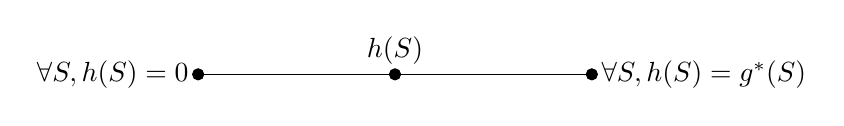
\begin{tikzpicture}
        % Disegna il segmento AB
        \draw[-] (0,0) -- (5,0);
        
        % Punti A, B e C
        \filldraw[black] (0,0) circle (2pt) node[left] {$\forall S, h(S) = 0$}; % Punto A
        \filldraw[black] (5,0) circle (2pt) node[right] {$\forall S, h(S) = g^*(S)$}; % Punto B
        \filldraw[black] (2.5,0) circle (2pt) node[above] {$h(S)$}; % Punto C al centro
    \end{tikzpicture}
\end{center}

Per progettare un'euristica, come abbiamo detto, è necessario non solo che sia ammissibile ma che la sua computazione sia efficiente (computata in tempo costante).
Chiaramente, più è efficiente l'euristica, meno stretta è, quindi dobbiamo trovare il compromesso giusto per avere una buona euristica.
Tale ha come estremi:
\begin{itemize}
    \item L'Estremo sinistro (caso in cui l'euristica è \textbf{triviale})
    \item L'Estremo destro (caso in cui è il problema ad essere \textbf{triviale} e l'euristica conosce già il percorso completo)
\end{itemize}
Realizzare una buona euristica per A* ci permette di diminuire di molto la dimensione degli alberi e permette di risparmiare tempo e spazio occupati, quindi il nostro obiettivo è di ottenere 
l'euristica migliore, ossia:\\
Dati $h_1, h_2 $ euristiche tali che $\forall S, h_1(S) \leq h_2(S)$ allora $h_2$ domina $h_1$. Inoltre, anche se non per tutti gli S un'euristica domina l'altra,
è possibile creare un'euristica dominante su $h_1, h_2$, ossia:
\begin{equation*}
    h_3 = \max\{h_1, h_2\}
\end{equation*}
Un modo che abbiamo per progettare un'euristica è risolvendo un \textbf{Problema Rilassato}

\subsubsection{Problema Rilassato}
Dato un problema $P$, il suo rilassamento $\hat{P}$ è una sua versione più semplice, ottenuta \textit{rilassando} alcuni suoi vincoli;
per esempio, in una mappa, il problema rilassato della ricerca del percorso l'abbiamo ignorando tutti gli ostacoli, ipotizzando di poter attraversare gli edifici.
Per questo motivo vale che per ogni $S,U$ nodi e $a$ azione:
\begin{equation*}
    \hat{c}(S,a,U) \leq c(S,a,U)
\end{equation*}
Risolvere un problema rilassato può essere una buona euristica.

\subsubsection{Limiti di A*}
Il problema di A* è, essenzialmente, che è troppo rigido: nel caso in cui sulla frontiera vi siano MOLTI nodi tutti con un valore di $f$
molto simile, allora A* perderà molto tempo a espanderli tutti quanti. Può essere anche che un nodo arrivi all'ottimo in un certo numero di passi,
mentre un altro nodo ci arrivi con un numero di passi decisamente inferiore. La formulazione di A* più flessibile è il \textbf{Focal Search}

\subsection{Focal Search}
Per l'implementazione del Focal Search è necessario implementare una nuova euristica $\hat{h_F}(n)$ che stima il costo \textbf{computazionale} (e non in termini di passi)
per raggiungere un goal. Questa euristica poi, rispetto all'euristica $h$, deve \textbf{sovrastimare} (quindi essere pessimista).
Possiamo risolvere diversi problemi NP-HARD con questa tecnica (vedi il TSP, potrebbe chiederlo all'esame)
